\subsection*{Pipeline} \label{s:pipeline}
The proposed portfolio optimisation uses (mostly well-known) techniques from Bayesian statistics and optimisation. The pipeline of our process is shown in Fig.\ \ref{fig:pipelinetikz}.
\usetikzlibrary{shapes, arrows.meta, positioning, fit, calc}

\definecolor{myblue}{HTML}{B4C8DC}   % Light blue (fill)
\definecolor{darkerblue}{HTML}{8C9FB5} % Border
\definecolor{textblue}{HTML}{0A2846}   % Optional dark blue text
\begin{figure}[!ht]
    \centering
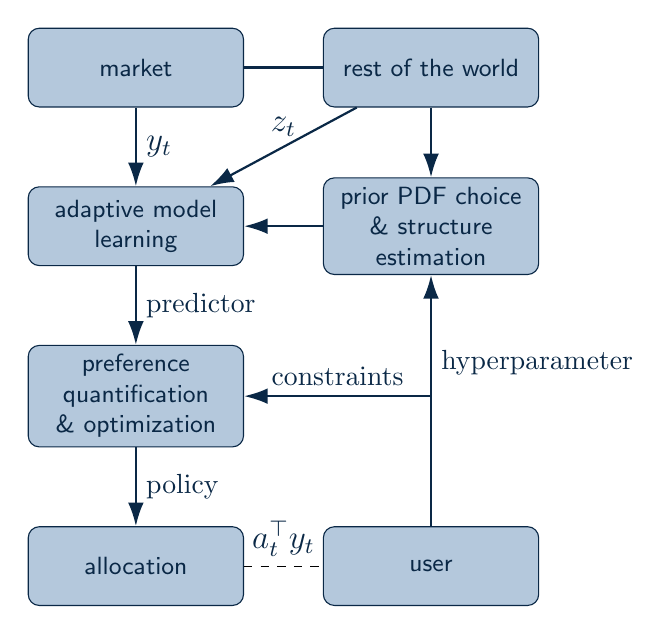
\begin{tikzpicture}[
    block/.style={rectangle, draw=textblue, fill=myblue, rounded corners,
                  text width=2.5cm, minimum height=1.0cm, align=center, font=\sffamily\small},
    decision/.style={diamond, draw=textblue, fill=darkerblue,
                     text width=2.5cm, minimum height=1cm, align=center, font=\sffamily\small},
    line/.style={draw, -{Latex[length=3mm, width=2mm]}, thick, textblue},
    textlabel/.style={pos=0.5, font=\sffamily\tiny, textblue},
    every node/.style={text=textblue}
]

    % Nodes
    \node (market) [block] {market};
    \node (rest_of_world) [block, right=1cm of market] {rest of the world};
    \node (model) [block, below=1cm of market] {adaptive model learning};
    \node (opt_prior) [block, right=1cm of model] {prior PDF choice \& structure estimation};
    \node (LQR) [block, below=1cm of model] {preference quantification \& optimization};
    \node (opt_alg) [block, below=1cm of LQR] {allocation};
    \node (user) [block, below=of opt_prior, right=of opt_alg] {user};

    % Connections
    \draw [line] (market.south) -- node[textlabel, right, font=\large] {$y_t$} (model.north);
    \draw [line] (opt_prior.west) -- (model.east);
    \draw [line] (rest_of_world) to node[textlabel, above, pos=0.5, font=\large] {$z_t$} (model);
    \draw [line] (model.south) -- node[textlabel, right, font=\normalsize] {predictor} (LQR.north);
    \draw [line] (LQR.south) -- node[textlabel, right, font=\normalsize] {policy} (opt_alg.north) ;

    % dashed line of returns to user
    \draw [dashed] (opt_alg.east) -- node[textlabel, above, pos=0.5, font=\large] {
$a_{t}^{\top}y_{t}$} (user.west);

    % Two-way arrow for Market and Rest of the World
    \draw [line, -] (market.east) -- (rest_of_world.west);

    % User loops
    \draw [line] (user.north) -- (opt_prior.south) node[textlabel, right, pos=0.65, font=\normalsize] {hyperparameter};
    \draw [line] (user.north) |- (LQR.east) node[textlabel, left, pos=0.1, above, pos=0.75, font=\normalsize] {constraints};

    % Feedback from LQR
    \draw [line] (rest_of_world.south) --(opt_prior.north);

\end{tikzpicture}
   \caption{\emph{Solution pipeline}:
   The market produces the observed $y_{t}$, which are returns of assets in the user's portfolio at time $t$. The rest of the world, which preserves past market data, gives information $z_{t}=(a_{t},x_{t-1})$ potentially useful for predicting the said returns. Data serves to model structure estimation, choice of Bayesian prior and forgetting. The learned model $(\mbox{available knowledge})\rightarrow y_{t}$ also serves for a quantitative expression of the user's wishes and for the optimal allocation $a_{t}$ of the funds before $y_{t}$ realisation. After it, the user receives the return $a_{t}^{\top}y_{t}$.
   }
    \label{fig:pipelinetikz}
\end{figure} 